\chapter{代码劫持方案的分析与设计}

上一章描述了针对VxWorks镜像的两种代码插入方式,
本章将描述如何在代码插入的基础上,
对目的函数进行劫持。
从而当该函数被调用时,我们插入的代码将得到执行。
插入代码执行完毕后,返回被劫持的函数,
而不会影响整个系统的正常运行。

劫持的思路有两种。
一种是劫持系统入口点,如图\ref{hijack1}所示。
另一种是劫持某一函数,如图\ref{hijack2}所示。

\begin{figure}[h!]
    \centering
    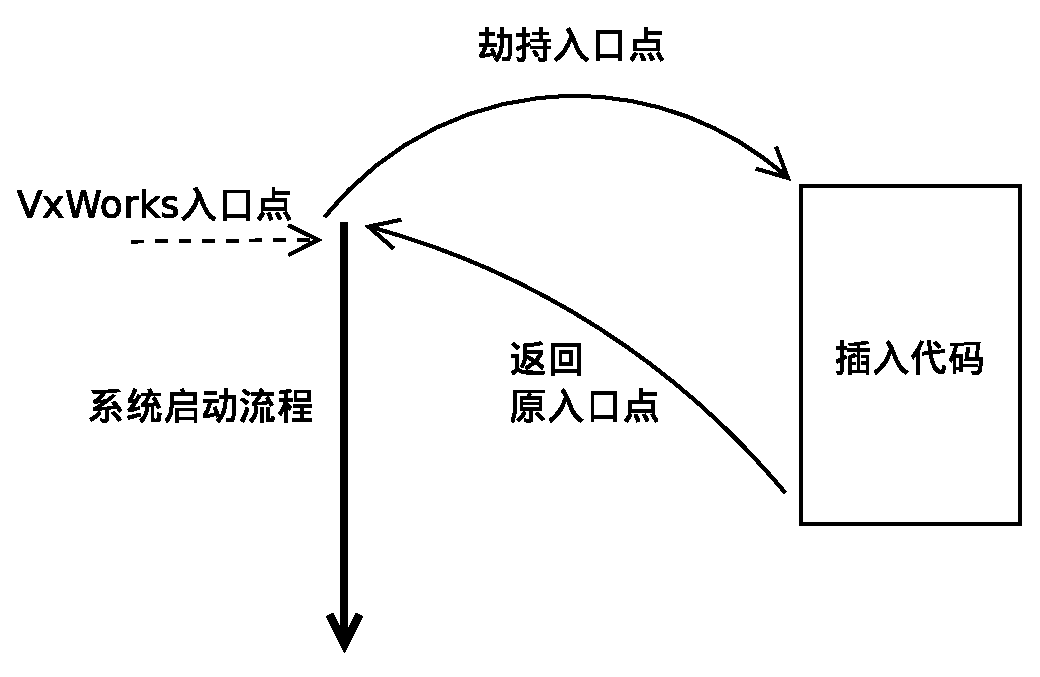
\includegraphics[width=0.55\textwidth]{figure/hijack1.eps}
    \caption{VxWorks入口点劫持思路}
    \label{hijack1}
\end{figure}

\begin{figure}[h!]
    \centering
    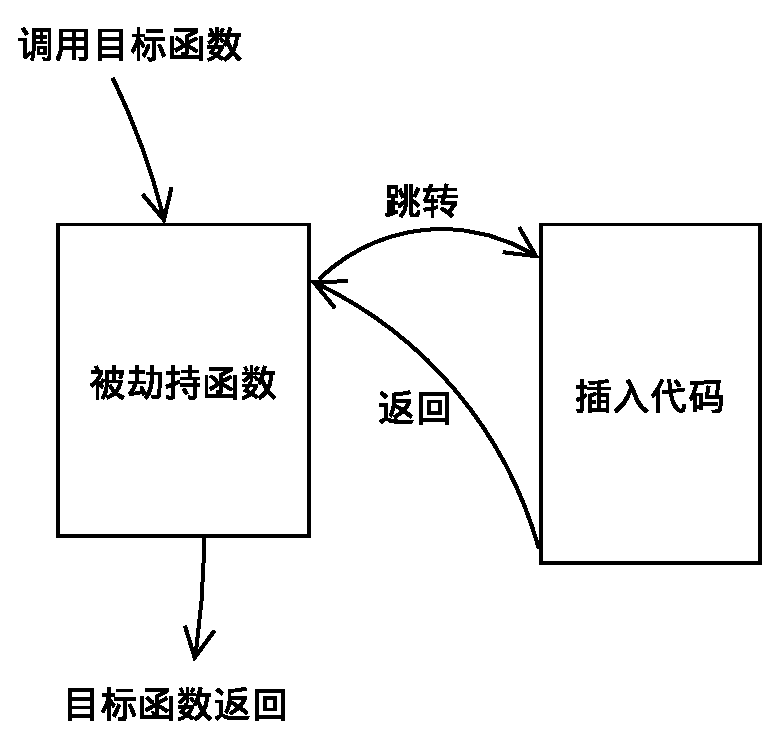
\includegraphics[width=0.4\textwidth]{figure/hijack2.eps}
    \caption{VxWorks函数劫持思路}
    \label{hijack2}
\end{figure}


%%%%%%%%%%%%%%%%%%%
%%%%%%  4.1  %%%%%%
%%%%%%%%%%%%%%%%%%%
\section{VxWorks系统镜像种类}

VxWorks的系统映像分为三种类型,
每一种映像类型都对应不同的加载方式。

\begin{itemize}
  \item 可加载的映像类型
\end{itemize}

可引导型映像需要一段引导代码才能装载到RAM中,
然后才能开始执行。


\begin{itemize}
  \item 基于ROM的映像类型,
\end{itemize}

这类镜像首先把自己从ROM或者Flash中
装载到RAM中,然后启动运行。

\begin{itemize}
  \item ROM驻留的映像类型
\end{itemize}

这类镜像与基于ROM的映像类型很相似,
但是它在拷贝自身的时候只拷贝数据段,
代码段仍然驻留在ROM中。
适用于RAM较小的一些嵌入式系统,
但运行速度会比较慢。

我们执行插入的对象是可加载的映像类型。
这类映像本身其实是一个ELF文件,
而不是平坦的二进制文件。
其加载过程由一个加载程序(通常称为bootloader)来完成。

%%%%%%%%%%%%%%%%%%%
%%%%%%  4.2  %%%%%%
%%%%%%%%%%%%%%%%%%%

\section{VxWorks系统启动调用流程}

虽然我们的插入工作仅针对ELF文件来进行,
并不修改bootloader的工作方式。
但了解bootloader程序的工作方式是有必要的。
就像在Linux下想要劫持ELF文件调用的共享库,
需要熟悉加载器和动态链接器如何工作一样。

如图\ref{boot}所示,VxWorks可加载型镜像的启动
主要有三个步骤(不考虑bootloader被压缩的情况):

\begin{figure}[h!]
    \centering
    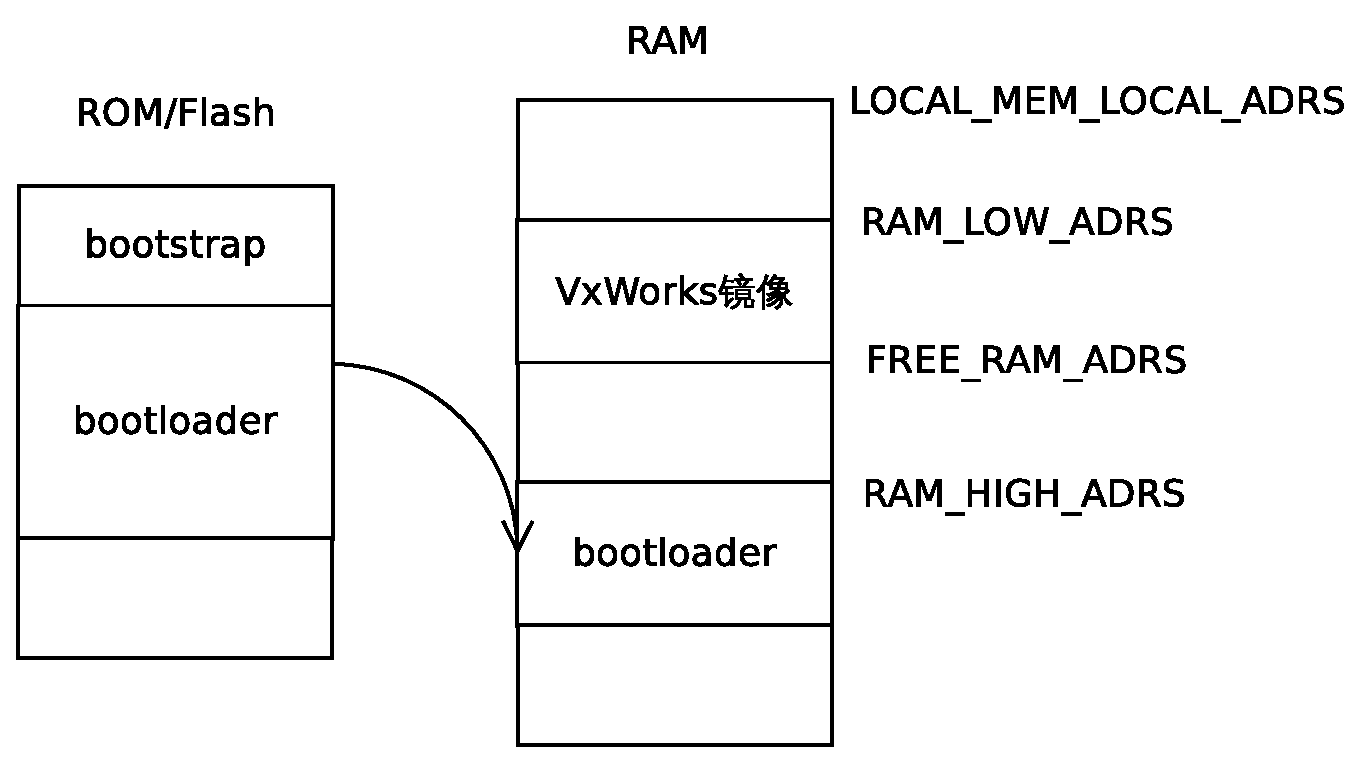
\includegraphics[width=0.68\textwidth]{figure/boot.eps}
    \caption{可加载型VxWorks镜像的启动}
    \label{boot}
\end{figure}

1、系统上电后,执行bootstrap的代码。
该程序进行一些基本的硬件初始化,
并负责将引导程序bootloader加载到
RAM中的RAM\_HIGH\_ADRS处。

2、系统跳转到RAM中,执行bootloader的代码,
该程序进行一些初始化工作之后,
通过网络或其他途径下载可加载型VxWorks镜像,
并加载到RAM中的的RAM\_LOW\_ADRS处。

3、镜像加载完毕后,
跳转到RAM中VxWorks的第一条指令处,
开始进行内核初始化。完成后启动应用程序。

系统初始化开始后,会调用一系列的函数用于初始化。
如图\ref{init}所示。

\begin{figure}[h!]
    \centering
    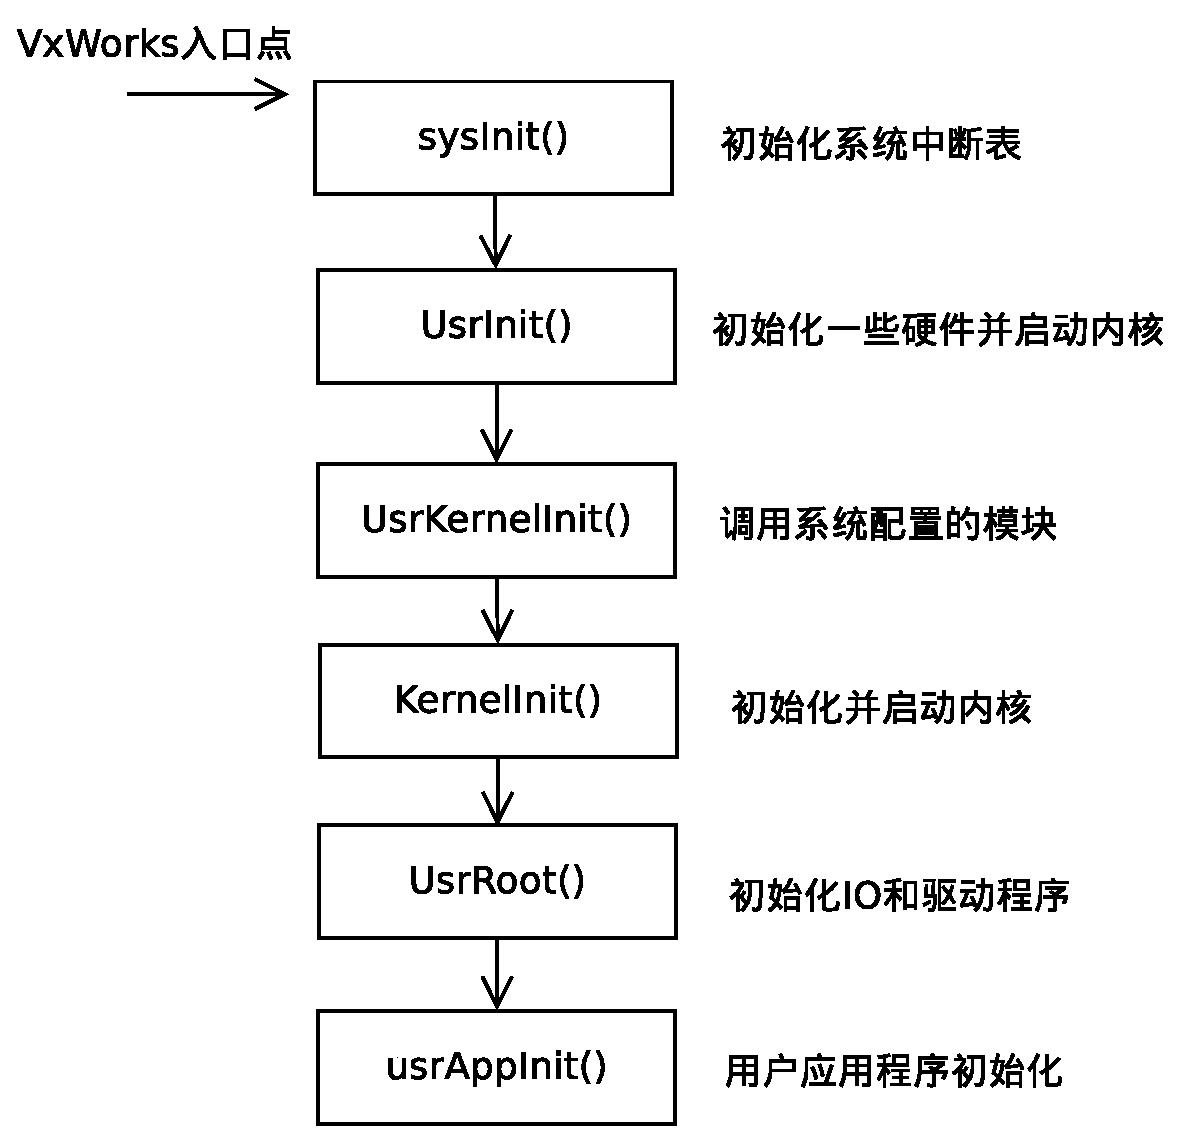
\includegraphics[width=0.55\textwidth]{figure/init.eps}
    \caption{VxWorks初始化函数调用流程}
    \label{init}
\end{figure}

由图可知,从VxWorks入口点开始,进行了一些硬件方面的初始化工作。
如果像在Linux下那样直接劫持入口点的话,
我们的代码可能不能正常运行,例如不能正常使用堆栈。
因此,函数的劫持应该有以下两个原则:

1、如果想要在系统启动后自动执行插入代码,
应劫持usrAppInit函数

2、如果希望在某函数被调用执行被插入代码,
应该在该函数头部插入跳转。

%%%%%%%%%%%%%%%%%%%
%%%%%%  4.3  %%%%%%
%%%%%%%%%%%%%%%%%%%
\section{VxWorks下代码劫持方案设计}


经过前文论述,已经证明,
在VxWorks下进行代码劫持其实只有一种情况,
即劫持某一个函数的入口。
本节在\label{section_hijcak}介绍的技术的基础上,
提出两种在VxWorks下可行的函数劫持方案,分别是直接跳转
和间接跳转。


\subsection{直接跳转及其可行性证明}

直接跳转类似\ref{sub_jmp}中介绍的跳转方案。
我们发现,一个由gcc编译产生的ELF文件中,
每个函数开头的几条指令和结尾的指令都是相似的。
一般函数体都形如代码\ref{function}所示。

\begin{lstlisting}[
  language={[x86masm]Assembler},
  caption={一般的x86函数体},
  label={function},
]
push ebp
mov ebp, esp
sub esp, ??h            ;函数体开头的三条指令,保存ebp,构建栈帧,分配空间。

……
……                      ;函数体中间部分。

mov esp,ebp
pop ebp
ret                     ;回收栈帧,取出ebp,返回上一级函数。
\end{lstlisting}

函数体都分为三个部分。
对于几乎每个函数来说,
它们的开头的三条指令和结尾的三条指令(有时是两条,为leave和ret指令)
几乎都是一样的。
这无形中为劫持函数提供了一个方便之处。

我们使用一个例子来说明这一劫持方案。
假设现有两个函数分别为A和B,
A为被劫持的函数,
B为用于劫持A的插入函数。
在劫持之前,
他们的函数体如图\ref{ab0}所示。

\begin{figure}[h!]
    \centering
    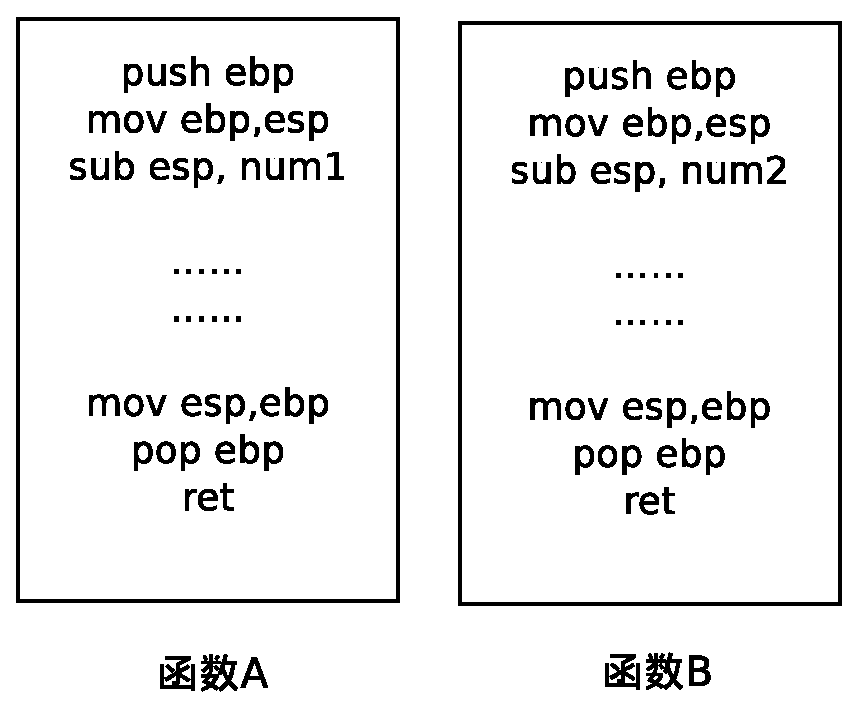
\includegraphics[width=0.44\textwidth]{figure/ab0.eps}
    \caption{修改前的函数A和函数B}
    \label{ab0}
\end{figure}

利用直接跳转法进行修改,修改后的两个函数结果如图\ref{ab1}所示。

\begin{figure}[h!]
    \centering
    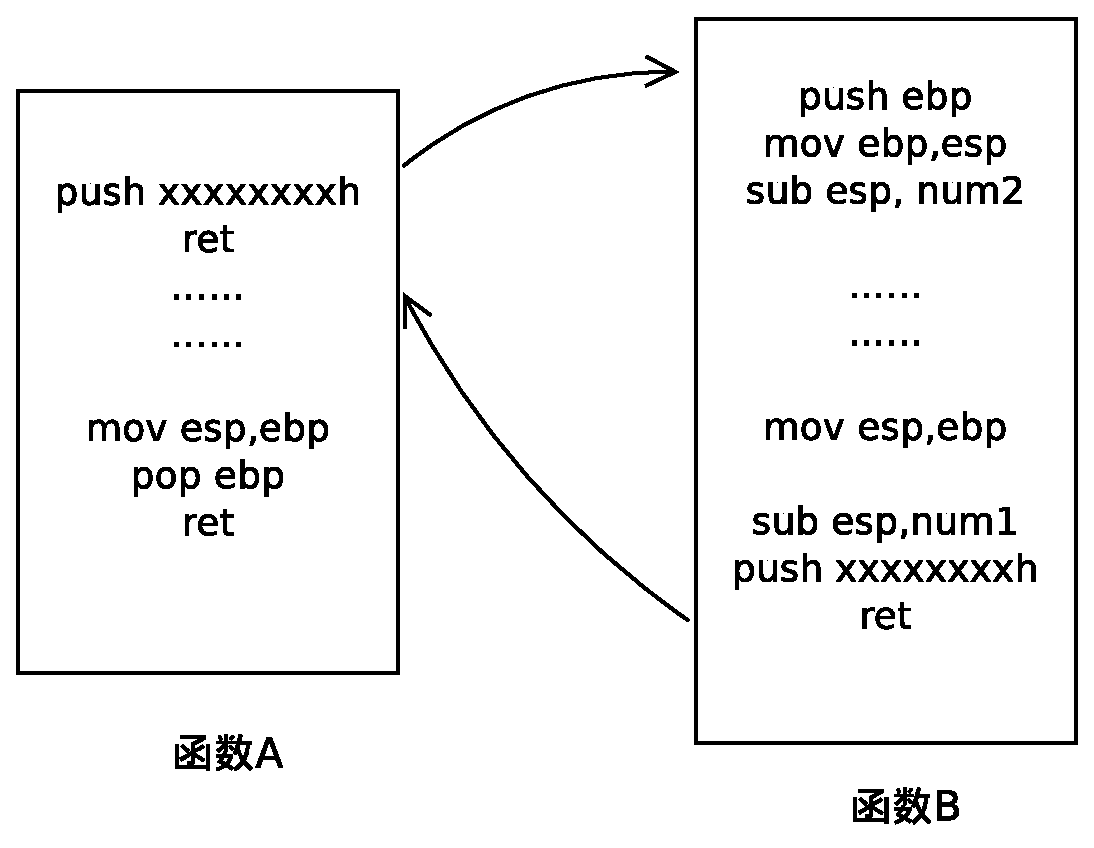
\includegraphics[width=0.58\textwidth]{figure/ab1.eps}
    \caption{修改后的函数A和函数B}
    \label{ab1}
\end{figure}

劫持算法如下:

1、修改A函数的前三条指令(6字节)为push+ret指令(6字节),目的是跳转到
B函数的第一条指令。

2、在B函数的ret指令前,添加两条指令:

第一条为A函数原来的第三条指令;

第二条为push指令,push内容为A函数的第四条指令的地址。

下面从指令执行流和堆栈、寄存器恢复的角度,
简要证明这种劫持方式的正确性:

1、控制流进入A函数时,还没有使用任何寄存器。
因此在B中可以使用任意的调用者保存寄存器(eax等)。
而在B中编译生成的代码会保存被调用者保存寄存器(ebx等)。
故寄存器不会因为函数劫持而被污染。

2、B中的倒数第四条指令,即mov指令,
恢复了在B中发生变化的esp寄存器;
而B中的开头两条指令和在倒数第三条添加的sub指令,
刚好恢复了A中删掉的三条指令。
故A的堆栈没有因为函数劫持而被污染。

3、A中因为push+ret指令跳转到了B中,
但最后又在B的最后跳回了A中。
因此指令执行流最后也被复原。

综上所述,从函数A的的角度看,
堆栈、寄存器和指令执行流都没有
因为函数的劫持而发生变化。
因此B的代码相当于透明地插入到了A的开头部分。

\subsection{间接跳转及其可行性证明}

上一条中使用的劫持方法,由被劫持函数A,
直接跳转到劫持函数B中。
为此付出的代价是仅仅是需要对B的结尾几条指令进行修改,
以恢复A的栈帧。

然而这种方法仍然存在几种不足之处:

1、插入的位置仅限于函数体的开头。

2、需要小心的修改劫持函数的指令。如果需要插入大量函数,工作量较大。

本条提出一种新的劫持思路,
即在使用一个中间层的思路,我们称这个中间层为proxy。
这需要我们插入两部分代码,一部分为proxy,一部分为劫持函数。

proxy劫持的原理非常简单。
函数劫持无非就是要在不污染原函数堆栈和寄存器的情况下,
改变指令的执行流。
为了能够更从容地保存和恢复寄存器和堆栈,
我们把这部分工作从劫持函数中分离出来,移到proxy中进行。

像???????????中一样,同样有两个函数分别为A和B,
B的任务是要劫持函数A。
利用proxy进行劫持的原理如图\ref{ab2}所示。

\begin{figure}[h!]
    \centering
    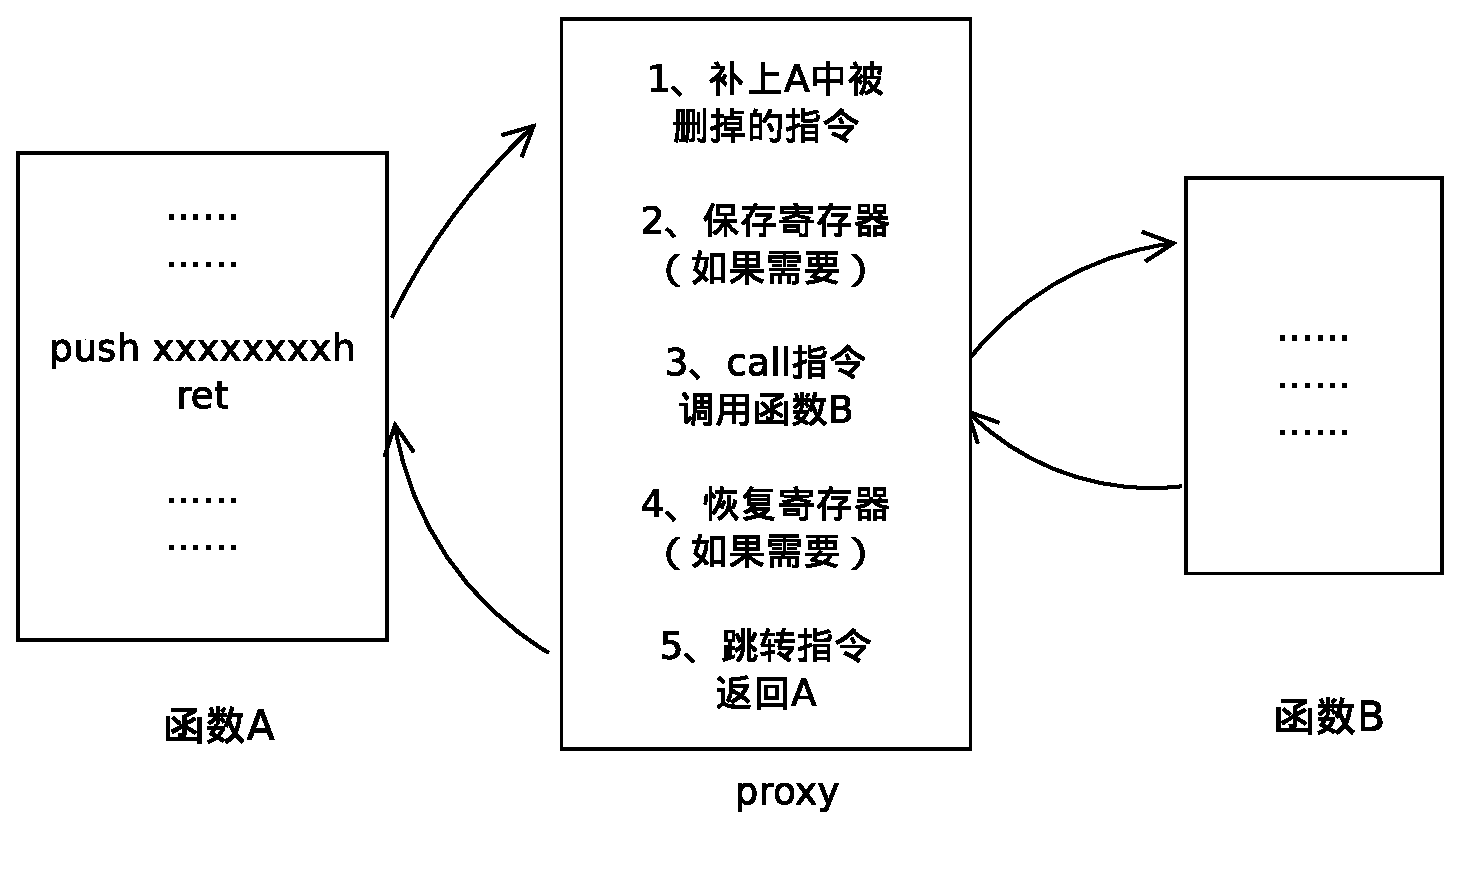
\includegraphics[width=0.76\textwidth]{figure/ab2.eps}
    \caption{使用proxy劫持函数原理}
    \label{ab2}
\end{figure}

在这一方法中,我们可以把A中的任意位置的进行劫持,
只需要修改相应位置为push+ret指令即可
(如果删掉的指令超过6字节,可用nop指令补齐)。

proxy要进行一系列的任务。
其中的核心任务是使用call指令调用函数B。
值得注意的是,由于对A的劫持可能来自任何一个地方,
当劫持位置之前,有调用者保存寄存器被使用的话,
B函数有可能会污染A中的调用者保存寄存器,例如eax。
因此在proxy中需要按照需要进行寄存器的保存和恢复。


使用这种方法,我们很自然地拥有了比较多的回旋的余地。
不必在狭小的B中进行寄存器保存的和恢复等工作。
在实际工作中,我们在编写B这样的劫持函数的时候,
就完全无需考虑任何有关劫持和插入的问题,
而是自由地使用高级语言编写,
然后像编译正常的程序一样编译即可。

\subsection{两种方案的对比和分析}

前文描述了两种在VxWorks下进行函数劫持的思路。
进行简单的对比和分析后,我们对两种方案的优劣总结如下:

1、直接跳转方案:

优点:插入代码量小。

缺点,逻辑比较复杂,劫持位置只能在函数体开头,对劫持函数的修改复杂。

2、间接跳转方案:

优点,逻辑清晰,劫持位置不受限制,proxy通用性强;

缺点,插入代码量教大。

在接下来的实际的实现工作中,
我们皆使用间接跳转方案。







